
\usetikzlibrary{shapes,arrows}

\tikzstyle{decision} = [diamond, draw, fill=blue!30, text badly centered, node distance=3.5cm, inner sep=3pt]
    
    %  text width=15em
\tikzstyle{block} = [inner sep = 10,rectangle, draw, fill=black!20, text centered, rounded corners, minimum height=3em,node distance=3cm]
    
\tikzstyle{fict_block} = [inner sep = 10,rectangle, draw, fill=magenta!40, text centered, rounded corners, minimum height=3em,node distance=3cm]
    
\tikzstyle{legend} = [inner sep = 0,circle, draw, fill=magenta!40, text centered, rounded corners, minimum height=2em,node distance=2.5cm]
    
\tikzstyle{line} = [draw, -latex']

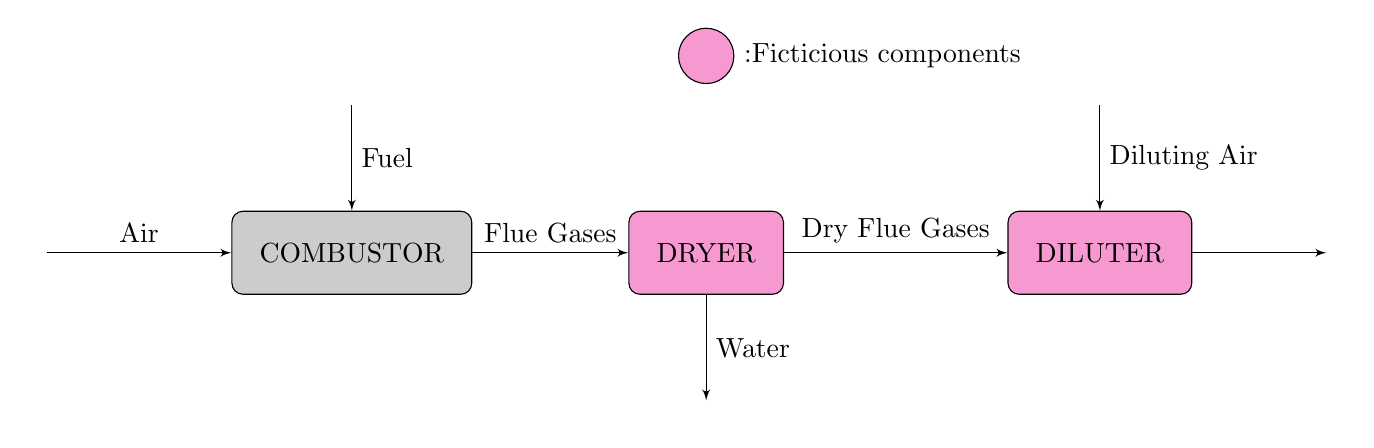
\begin{tikzpicture}
%[node distance = 1cm, auto]


\node [block] (combustor) {COMBUSTOR};
\node [fict_block,  right of=combustor,  align=center,  node distance=4.5cm] (dryer) {DRYER};
\node [fict_block,  right of=dryer,  align=center,  node distance=5cm] (diluter) {DILUTER};

\node [left of=combustor, node distance=4cm] (air) {}; 
\node [above of=combustor,node distance=2cm] (fuel) {};
\node [below of=dryer ,node distance=2cm] (water) {};
\node [above of=diluter,node distance=2cm] (dil) {};
\node [right of=diluter,node distance=3cm] (exit) {};

\path [line] (air) -- node[anchor=south] {Air} (combustor);
\path [line] (fuel) --  node[anchor=west] {Fuel} (combustor);
\path [line] (dryer) --  node[anchor=west] {Water} (water);
\path [line] (dil) --  node[anchor=west] {Diluting Air} (diluter);
\path [line] (diluter) --  node[anchor=west] {} (exit);

\path [line] (combustor) -- node[anchor=south] {Flue Gases}  (dryer) ;
\path [line] (dryer) -- node[anchor=south] {Dry Flue Gases} (diluter);
 
\node [legend, above of=dryer, label=0::Ficticious components]  (legend) {}  ;

\end{tikzpicture}